\chapter{The renewed panel SDK}
The new front-end and back-end codebase provide an interface developer with a
whole new set of tools.

\section{Packages available to panel developers}
The set of pre-made tools available to developers has vastly expanded.

Not only does this mean a more rich set of tools are developed internally,
developers can now also find and include tools they find on the web.

This will provide a way to get the framework capabilities to evolve as time
goes on.

\subsection{Bower Components}
All libraries, web components, sources, \ldots that are not developed in-house
are housed in the bower-components package.
The name is derived from the package manager used to pull in these resources,
called `bower` (\url{http://bower.io/}).

The bower-components package contains a `bower.js` file that specifies the
dependencies to be pulled from the web.
Then the dependencies are compressed into a tarball. This is done to make sure
the package versions do not change unintentional, and new package versions can
be tested in a controlled manner.

Currently, the following elements are included in bower-components:

\begin{labeling}{vaadin-core-elementssss}
\item [\textbf{Polymer}] (\url{https://www.polymer-project.org/})
\item [\textbf{iron-elements}] (\url{https://elements.polymer-project.org/browse?package=iron-elements})
The iron-elements are a set of web components aiming to provide a basic set of
tools and enhancements to standard elements, for example to provide them with
data-binding capabilities.

These elements do not make assumptions about the used layout or styling, and are
expected to maintain a spartan view, if they render a view at all.

Iron-elements aim to extend basic html elements (e.g. <iron-input> to extend
<input>), provide façade elements for javascript functionality (e.g. <iron-ajax>
to easily make AJAX requests), or provide new functionality that would be
considered basic functionality (e.g. <iron-icon> to display an icon).
\item [\textbf{paper-elements}] (\url{https://elements.polymer-project.org/browse?package=paper-elements})
Paper-elements is a set of elements that focus on bringing Material Design\cite{materialdesign}
to web components.

Paper-elements aims to extend iron-elements with material design (e.g. <iron-input>
becomes <paper-input>), and introduce new elements that are unique to material
design (e.g. <paper-toast>)
\item [\textbf{gold-elements}] (\url{https://elements.polymer-project.org/browse?package=gold-elements})
Gold elements are input elements for specific use cases (e.g. email, phone numbers,
credit card numbers, \ldots).

They all extend the `paper-input` element and provide specific validation and
formatting functionality.
\item [\textbf{neon-elements}] (\url{https://elements.polymer-project.org/browse?package=neon-elements})
neon-elements are a set of Web Components designed to be façades for the
JavaScript animation API to make them available by purely writing HTML.

These elements do not use CSS Transitions, CSS Animations, or SVG, rather they
use the new Web Animations API (\url{https://www.w3.org/TR/web-animations/}).

These are among the most advanced Web Components in the packages available to
panel developers.
More info about their usage is provided here: \url{https://youtu.be/-tX0e29GQa4}.
\item [\textbf{platinum-elements}] (\url{https://elements.polymer-project.org/browse?package=platinum-elements})
Platinum-elements are a set of Web Components focused on providing a façade for
web-app capabilities like Service Workers, server push, and bluetooth connectivity.
\item [\textbf{jQuery}] (\url{https://jquery.com/})
\item [\textbf{moment.js}] (\url{http://momentjs.com/}) \\
JavaScript library for parsing, validating, manipulating, and formatting dates.
\item [\textbf{page.js}] (\url{https://visionmedia.github.io/page.js/}) \\
Micro client-side JavaScript router inspired by the Express router.
\item [\textbf{spectrum.js}] (\url{https://bgrins.github.io/spectrum/}) \\
Spectrum is a JavaScript colorpicker plugin using the jQuery framework.
\item [\textbf{juicy-jsoneditor}] (\url{https://github.com/Juicy/juicy-jsoneditor/})
\item [\textbf{cytoscape}] (\url{http://cytoscape.org/})
\item [\textbf{paper-datatable}] (\url{https://github.com/David-Mulder/paper-datatable})
\item [\textbf{vaadin-core-elements}] (\url{https://vaadin.com/elements}) \\
Vaadin-core-elements are a set of Web Components developed by Vaadin
(\url{https://vaadin.com}). It focused on developing Web Components for business
use cases like data grids, charts, iconsets, file uploaders, and specific user
interface elements like a modified dropdown and a date picker.
\item [\textbf{juicy-ace-editor}] (\url{https://github.com/Juicy/juicy-ace-editor/}) \\
Custom Element with Ace(\url{http://ace.c9.io/}) code editor.
\item [\textbf{file-saver.js}] (\url{https://github.com/eligrey/FileSaver.js/}) \\
FileSaver.js implements the HTML5 W3C saveAs() FileSaver interface in browsers that do not natively support it.
\item [\textbf{saveSvgAsPng}] (\url{https://github.com/exupero/saveSvgAsPng.git}) \\
Save SVGs as PNGs from the browser.
\item [\textbf{KaTeX}] (\url{https://github.com/Khan/KaTeX}) \\
Fast math typesetting for the web.
\end{labeling}

\subsection{common-elements}
The common-elements package is composed of a set of in-house developed Web Components.

The main focus of this package is to provide panel developers with frequently
used functionality. This includes server callbacks, custom input elements, etc.

Currently the Web Components bundled with common-elements are the following:
\begin{labeling}{cumulative-line-chartttt}

\item [\textbf{KaTeX-js}] Loads the katex.js library, used to render latex math in javascript
\item [\textbf{auto-update}] automatically updates server-side data
Note that it is very similar to ts-ajax. However ts-ajax only makes a request when you ask for it, auto-update implements an interval with which it will automatically and periodically make a request.
Example html in a panel:
\begin{verbatim}
<auto-update data="{{my_variable}}"
             callback="cpp_callback"
             handle-as="text"></auto-update>
<span>{{my_variable}}</span>
\end{verbatim}
\item [\textbf{color-picker}] polyfills the html5 color input.
This element will be a plain html5 color input element if supported. If not, it
will load spectrum.js and provide a color input via JavaScript.
\item [\textbf{command-input}] receives three values 'name', 'value', and 'type' and converts it into an appropriate input element.
Currently, command-input recognizes the following data types: number, int, long, unsigned int, unsigned long, short, unsigned short, string, double, and float.
Examples:
\begin{verbatim}
<command-input name="dinosaurs are great"
               value="true" type="bool"></command-input>
<command-input name="your_favorite_dinosaur"
               value="deinonychus"
               type="string"></command-input>
<command-input name="positive number"
               value="0"
               type="unsigned int"></command-input>
\end{verbatim}
\item [\textbf{fake-a}] is a Polymer element that behaves like an anchor (<a>) element, but does not follow the href and thus does not accidentally cause a page refresh.
Example:
\begin{verbatim}
<fake-a on-click="something">click me</fake-a>
\end{verbatim}
\item [\textbf{file-saver-js}] loads the file-saver.js library. Used to save files with javascript.
\item [\textbf{iron-flex-layout-attributes}] provide a simple way to use the css flexbox system.
It follows the same syntax as the `iron-flex-layout`, a guide for this syntax
is available here: \url{https://elements.polymer-project.org/guides/flex-layout}
\item [\textbf{key-value-pair}] is a simple element that takes a key and a value and presents it nicely.
Example:
\begin{verbatim}
<key-value-pair key="my key"
                value="my value"></key-value-pair>
\end{verbatim}
\item [\textbf{master-detail-layout}] implements a responsive master-detail layout
When on a large enough screen, the master and detail view are displayed side to side. When on a small device, either the master or the detail view is shown, and the user can switch between them
Example:
\begin{verbatim}
<master-detail-layout>
  <div master>I am the master view</div>
  <div detail>I am the detail view</div>
</master-detail-layout>
\end{verbatim}
\item [\textbf{math-equation}] element that takes latex math input and renders it as a proper equation
\item [\textbf{moment-js}] loads the moment.js library
\item [\textbf{page-js}] loads the page.js library
\item [\textbf{relative-time}] takes a date string and converts it to a relative time (ex: 2h ago) using moment.js
Example:
\begin{verbatim}
<relative-time date="Fri Feb 12 2016 16:30:35 GMT+0100 (CET)">
</relative-time>
\end{verbatim}
\item [\textbf{reset-css}] makes an element follow the AjaXell theme.
When other elements use this element, that element will be enriched with theme
directives (colors, sizes, fonts, \ldots).
\item [\textbf{responsive-behavior}] extends an element with material design breakpoints.
It implements the breakpoints from material design. This behavior will give the
element a style tag corresponding to the current screen size (extra-small, small,
medium, large, extra-large), this can be used to style an element.
\item [\textbf{save-svg-as-png}] loads the saveSvgAsPng.js library. It converts an SVG tag to a png bitmap.
\item [\textbf{ts-ajax}] makes an ajax request to a specified callback.
It is very similar to auto-update, except for the fact that this doesn't have an interval, it only makes a request when you ask it to. Also not that the C++ callback event is 'OnClick' and not 'OnTime' as with auto-update.
Example html in a panel:
\begin{verbatim}
<ts-ajax data="{{my_variable}}"
         callback="cpp_callback"
         handle-as="text"
         auto></ts-ajax>
<span>{{my_variable}}</span>
\end{verbatim}
\item [\textbf{ts-colors}] Gives an element access to the material design color palette via attributes
\item [\textbf{ts-tree}] renders a tree structure from a given JSON.
\item [\textbf{cytoscape-import}] loads the cytoscape.js library


\item [\textbf{candlestick-chart}] renders a cumulative line chart
\item [\textbf{cumulative-line-chart}] renders a cumulative line chart using nvd3.js
\item [\textbf{cytoscape-import}] loads the cytoscape.js library
\item [\textbf{d3-import}] loads the d3.js library
\item [\textbf{discrete-bar-chart}] renders a cumulative line chart
\item [\textbf{focus-line-chart}] renders a line chart with focus area using nvd3.js
\item [\textbf{historical-bar-chart}] renders a cumulative line chart
\item [\textbf{horizontal-stacked-bar-chart}] renders a horizontally stacked bar chart using nvd3.js
\item [\textbf{line-chart}] renders a line chart using nvd3.js
\item [\textbf{multi-chart}] advanced chart element capable of rendering multiple charts as one
\item [\textbf{nvd3-chart-behavior}] the behavior that holds all common element code for NVD3-based chart elements
\item [\textbf{nvd3-import}] imports the nvd3.js library, a JavaScript charting library based on D3
\item [\textbf{parallel-chart}] renders a cumulative line chart
\item [\textbf{pie-chart}] renders a pie chart using nvd3.js
\item [\textbf{scatter-chart}] renders a scatter chart using nvd3.js
\item [\textbf{stacked-area-chart}] renders a stacked area chart using nvd3.js
\item [\textbf{stacked-bar-chart}] renders a stacked bar chart using nvd3.js
\item [\textbf{state-diagram}] renders a state diagram using cytoscape.js
\item [\textbf{sunburst-chart}] renders a sunburst chart using nvd3.js
\end{labeling}
This list is taken from \url{http://cell/ts/common-elements/index.html}

\subsection{JsonCpp}
\label{JsonCpp}
A panel developer will now use the C++ code primarily for data generation.
Therefore it should have some very good tools to send data to the client.

In the legacy codebase the way to put data in JSON format was by using a
BOOST Property Tree.
Unfortunately BOOST Property trees are not very adequate to generate JSON. They
for example don't support the notion of arrays\cite{boost_propertytrees}.

BOOST Property trees have been replaced in the new codebase by JsonCpp,
(\url{https://github.com/open-source-parsers/jsoncpp}), a lightweight library
specifically designed to render and interpret JSON strings.

JsonCpp allow for much more cleaner code.
Consider the following example:

This code creates an array of objects using BOOST. Note the fact developers have to
render the array manually. This can made code very messy if a developer would need an
array inside a property tree, the code stays relatively clean now because the
array is the root node.
\fvset{frame=single}
\begin{pyglist}[language=cpp,numbers=left,numbersep=5pt,fontsize=\small]
map<string, xdata::Serializable*> dummyParams = getOperation().getParamList();

out << "[";
for ( map<string,xdata::Serializable*>::iterator i = dummyParams.begin();
      i != dummyParams.end(); ++i ) {
  if (i != dummyParams.begin()) {
    out << ",";
  }
  boost::property_tree::ptree object;
  object.put("name", i->first);
  object.put("type", i->second->type());
  object.put("value", dummyParams [i->first]->toString());
  boost::property_tree::write_json(out, deviceTree);
}
out << "]";
\end{pyglist}
\fvset{frame=none}

Now consider the same array of objects, but this time created with JsonCpp.
Note that the code is much cleaner.
\fvset{frame=single}
\begin{pyglist}[language=cpp,numbers=left,numbersep=5pt,fontsize=\small]
map<string, xdata::Serializable*> dummyParams = getOperation().getParamList();

Json::Value root(Json::arrayValue);
for ( map<string,xdata::Serializable*>::iterator i = dummyParams.begin();
      i != dummyParams.end(); ++i ) {
  Json::Value input;
  input["name"] = i->first;
  input["type"] = i->second->type();
  input["value"] = dummyParams [i->first]->toString();
  root.append(input);
}
out << root;
\end{pyglist}
\fvset{frame=none}

\section{New Cell structure}
The cell folder structure looks as follows (see figure \ref{fig:filetree}).
The `src/common` folder contains all C++ code, except the header files.
Header files are kept in the `include` folder.
The `src/html` folder contains any front-end code that needs processing (e.g.
transpiling or minifying code). The result of any processing from this
folder will be put in the `html` folder.
The `html` folder also contains any static front-end code that needs no processing.

For more info about the processing from `src/html` to `html`, see chapter \ref{Grunt build system}.
\begin{figure}
  \centering
  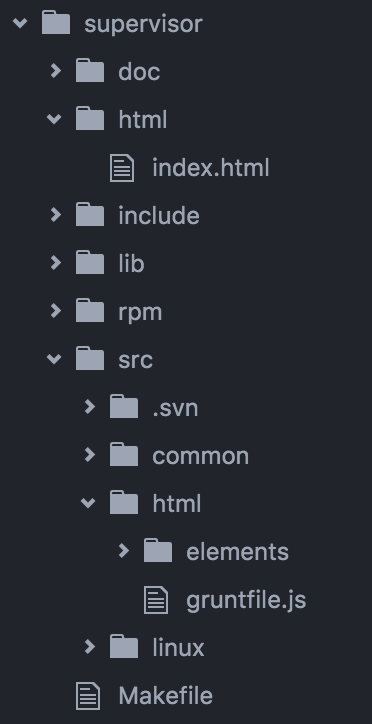
\includegraphics[width=.3\textwidth]{images/filetree}
  \caption{Trigger Supervisor folder stucture}
  \label{fig:filetree}
\end{figure}

\section{Separation of Concerns}
\label{Separation of Concerns}
SoC is a design primitive, dictating a modular design of the software. This has
been implemented in three ways.

Firstly, different syntaxes now are housed in their own files. This allows for
significantly less messy code and enables us to implement specific optimizations
for each language (for example a CSS pre- and post-processor).

Secondly, the developer is not limited to one source file for each syntax. If
circumstances would make some code easier to manage if it is housed across
multiple files this is now possible. An example of this would be a panel with
multiple specialized sections. Separating these sections will make the code
easier to read and maintain.

Thirdly, this approach pushes developers to separate data from markup. This is
a very good thing as it causes the code to once again be much more readable.
By having the C++ code only produce the necessary data and putting all rendering
and interaction on the front-end, developers can also safely replace rendering logic or
user interaction flow without having to worry about data generation.

\section{Grunt build system}
\label{Grunt build system}
During development of the front-end code. Code is kept in multiple files (for
the SoC principle).

Instead of loading all the separated files individually at runtime, they will
instead be compiled together at compile-time. This will improve loading speeds.
The tool used to do this is Grunt
\url{http://gruntjs.com/}, a task runner built on nodeJS that is used to process
front-end code languages. It is currently a popular tool to compile,
minify, lint, unit-test, etc. front-end code before it is put in production.
It has very wide community adoption, which results in a very rich set of tools
available for use.

Now that every code language is housed in specialized files, some
optimizations on them can run at compile-time. The main objective of these optimizations
is to achieve as much browser compatibility as possible.

\subsection{JavaScript processing}
In order to ensure compatibility with all required browsers all JavaScript code
is transpiled by Babel \url{https://babeljs.io/}. This will ensure that newer syntax,
like ECMAScript 2016 (ES7), will be transpiled into a more compatible equivalent.

Also the JavaScript code will be transpiled by UglifyJS
\url{https://github.com/mishoo/UglifyJS}. This will implement various code
optimizations\cite{UglifyJSCompressor} making the code faster.
% \subsubsection{Linting}
% \subsubsection{Transpilation of ES6}
% \subsubsection{Uglification}
\subsection{CSS processing}
\subsubsection{SASS}
Developers are given the possibility to write SASS code, an extension of the CSS
syntax, that will be transpiled into CSS on compile-time using libsass
\url{http://sass-lang.com/libsass}.

\subsubsection{Autoprefixer}
Also Grunt will automatically add vendor-specific prefixes to CSS properties to
maintain the required browser compatibility using a tool called autoprefixer
\url{https://github.com/postcss/autoprefixer}.
\subsection{HTML processing}
No processing is done on the html code except for the fact that it is inlined.
\subsubsection{Inliner}
Any css link tag or script tag is inlined (i.e. the contents of the referenced
file read and inserted in the document) when the url in that tag contains
`\_\_inline=true`.

\section{Templates}
To assist developers when creating new interfaces, a set of template files and
scripts have been developed.

Where appropriate, a script `new-element.js` is present. A developer can execute
this command to create a new element containing html, sass, and javascript code,
all with inline documentation and a demo page.

\section{Panel registration system}
An interface consists of multiple libraries. Each of these could possibly contain
element definitions (e.g. the AjaXell library has elements concerning things like
session management).

To allow any loaded library to declare its own Web Components, a panel
registration system is included in the AjaXell libary.

It allows a developer to register any custom elements he developed in his cell
like so:
\fvset{frame=single}
\begin{pyglist}[language=cpp,numbers=left,numbersep=5pt,fontsize=\small]
void <package-name>::Cell::init()
{
  getContext()->addImport("/<package-path>/html/elements/elements.html");
}
\end{pyglist}
\fvset{frame=none}
With the `elements.html` file containing element definitions, either in eager
loading or in lazy loading syntax.

\subsection{Eager loading and lazy loading}
Depending on the content of the `elements.html` file, the element definitions
will either be loaded eagerly (i.e. at page load time) or lazy (i.e. when they
are needed). Of course a developer is encouraged to implement the lazy loading
approach, as it will decrease initial page loading times.

The eager loading approach is a list of HTML imports.
\fvset{frame=single}
\begin{pyglist}[language=html,numbers=left,numbersep=5pt,fontsize=\small]
<link rel="import" href="my-first-element/my-first-element.html" >
<link rel="import" href="my-second-element/my-second-element.html" >
\end{pyglist}
\fvset{frame=none}

While the lazy loading approach consists of a custom function provided by AjaXell.
\fvset{frame=single}
\begin{pyglist}[language=html,numbers=left,numbersep=5pt,fontsize=\small]
<script>
var base = document._currentScript.baseURI;
base = base.substring(0, base.lastIndexOf("/") + 1);

LazyLoad({
  base: base,
  provides: {
    "my-first-element": "my-first-element/my-first-element.html",
    "my-second-element": "my-second-element/my-second-element.html"
  }
})
</script>
\end{pyglist}
\fvset{frame=none}
